\documentclass[10pt, spanish, pdftex]{../.template/template}	

%%%%%%%%%%%%%%%%%%%%%%%%%%%%%%%%%%%%%%%%%%%%%%%%%%%%%%%%
%               UC3M Work report template              %
%           Universidad Carlos III de Madrid           %
%              Author: Aitor Alonso Núñez              %
%              Last update: March 8, 2018              %
%%%%%%%%%%%%%%%%%%%%%%%%%%%%%%%%%%%%%%%%%%%%%%%%%%%%%%%%

%%%%% Preamble %%%%%
\usepackage{fancyhdr}				% To add header and footer
\usepackage{graphicx}				% To add images
\usepackage{caption}				% To add captions
\usepackage{subcaption}				% To add subcaptions
\usepackage{lipsum}					% Example Lorem ipsum text
\usepackage[hidelinks]{hyperref}	% Index elements works as cross references. Also functional links to internet pages
\usepackage{nameref}				% Allow to add labels with \label{name} which can be reference with \nameref{name}
\author{Aitor Alonso Núñez}			% This is me!

\usepackage{listings}
\graphicspath{{images/}}
\usepackage{tikz}
\usetikzlibrary{arrows, automata, chains, matrix}
\usepackage{adjustbox}
\usepackage[table,xcdraw]{xcolor}
\usepackage{bm}


\newcommand{\namerefs}[1]{\textit{\underline{\color{uc3mNewBlue}\nameref{#1}}}}
\newcommand{\customref}[2]{\textit{\underline{\color{uc3mNewBlue}\hyperref[#1]{#2}}}}

%%%%% Coauthors info %%%%%
%%[1-2] If you want to show coauthors email address on the title page, enable \emailtrue. Otherwise, enable \emailfalse
\emailtrue
% \emailfalse
%% If coauthors are between 1 and 2 uncomment these options. Comment it otherwise.
%% You can leave empty keys {} if you need to.
\coauthorstwotrue		% coauthors two = true
\coauthorsthreefalse	% coauthors three = false
\coauthorsfourfalse		% coauthors four = false
\coauthorstwo{Aitor Alonso Núñez}{NIA 100346169}{Gr. 83}{Daniel Gak Anagrov}{NIA 100318133}{Gr. 83}
%%[3] If you enabled \emailtrue, uncomment the option below
\emailstwo{100346169@alumnos.uc3m.es}{100318133@alumnos.uc3m.es}

%% If coauthors are between 1 and 2 uncomment these options. Comment it otherwise.
%% You can leave empty keys {} if you need to.
% \coauthorstwofalse		% coauthors two = false
% \coauthorsthreetrue		% coauthors three = true
% \coauthorsfourfalse		% coauthors four = false
% \coauthorsthree{Name1 Lastname1}{NIA 100XXXXXX}{Gr. XX}{Name2 Lastname2}{NIA 100XXXXXX}{Gr. XX}{Name3 Lastname3}{NIA 100XXXXXX}{Gr. XX}
%% If you want to show on the title page the email address of these coauthors uncomment the next options
%% and comment \emailfalse. In other case, comment everything except \emailfalse
% \emailsthree{email1@domain.tld}{email2@domain.tld}{email3@domain.tld}

%%[4] If coauthors are between 1 and 2 uncomment these options. Comment it otherwise.
%% You can leave empty keys {} if you need to.
% \coauthorstwofalse		% coauthors two = false
% \coauthorsthreefalse		% coauthors three = false
% \coauthorsfourtrue		% coauthors four = true
% \coauthorsfour{Name1 Lastname1}{NIA 100XXXXXX}{Name2 Lastname2}{NIA 100XXXXXX}{Name3 Lastname3}{NIA 100XXXXXX}{Name4 Lastname4}{NIA 100XXXXXX}
%% If you want to show on the title page the email address of these coauthors uncomment the next options
%% and comment \emailfalse. In other case, comment everything except \emailfalse
% \emailsfour{email1@domain.tld}{email2@domain.tld}{email3@domain.tld}{email4@domain.tld}


%%%%% Basic data about the document (Degree, subject, title, campus, page number custom text) %%%%%
\documentdata{Grado en Ingeniería Informática}{Aprendizaje Automático}{Tutorial 4: Aprendizaje por refuerzo}{Página }

%%%%% Page style %%%%%
\header
\footer
\pagestyle{fancy}
\begin{document}

%%%%% Page title %%%%%
\titleMain

%%%%% Index %%%%%
\tableofcontents 	% We add the index
\newpage 			% And before index we start on a new page

%%%%% CONTENIDO DEL DOCUMENTO %%%%%
%% VERY IMPORTANT!!! On the first line of this .tex file, select Spanish or English language to coincide with document text language
\section{Introducción}
\p{El presente documento responde a las preguntas realizadas en el \textit{tutorial 4: Aprendizaje por refuerzo} de la asignatura Aprendizaje Automático. Asimismo, detalla el trabajo que hemos desarrollado durante el tutorial y argumenta cada una de las decisiones y respuestas realizadas.}

\section{MDP determinista}
\subsection{7. Ilustración del modelo}
\p{Hemos nombrado a cada estado posible del MDP como XY, donde X es la fila del laberinto (comenzando por la fila de arriba en cero) e Y es la columna del laberinto (comenzando por la columna de la izquierda en cero). De esta forma, el agente solo puede transicionar a estados cuyo nombre difiere solo en una cifra respecto al estado actual.}

\begin{figure}
% Grid
\begin{adjustbox}{valign=m,minipage={0.4\linewidth}}
    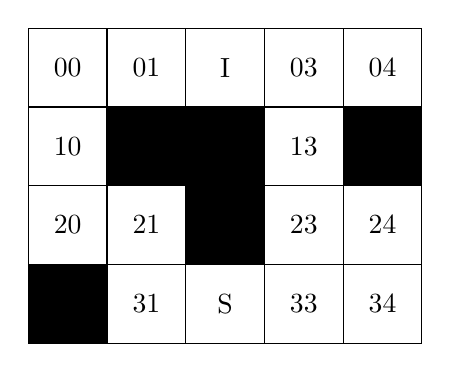
\begin{tikzpicture}
        % Pintar grid
        \draw[step=1cm,black] (0,0) grid (5,4);
        % Poner los muros de negro (casillas negras)
        \fill[black] (0,0) rectangle (1,1);
        \fill[black] (1,2) rectangle (2,3);
        \fill[black] (2,2) rectangle (3,3);
        \fill[black] (2,1) rectangle (3,2);
        \fill[black] (4,2) rectangle (5,3);
        % Texto de las casillas
        \node at (0.5,3.5) {00};
        \node at (1.5,3.5) {01};
        \node at (2.5,3.5) {I};
        \node at (3.5,3.5) {03};
        \node at (4.5,3.5) {04};

        \node at (0.5,2.5) {10};
        \node at (3.5,2.5) {13};

        \node at (0.5,1.5) {20};
        \node at (1.5,1.5) {21};
        \node at (3.5,1.5) {23};
        \node at (4.5,1.5) {24};

        \node at (1.5,0.5) {31};
        \node at (2.5,0.5) {S};
        \node at (3.5,0.5) {33};
        \node at (4.5,0.5) {34};
    \end{tikzpicture}
    % \hspace{1cm}
\end{adjustbox}
% MDP
\begin{adjustbox}{valign=m,minipage={0.4\linewidth}}
    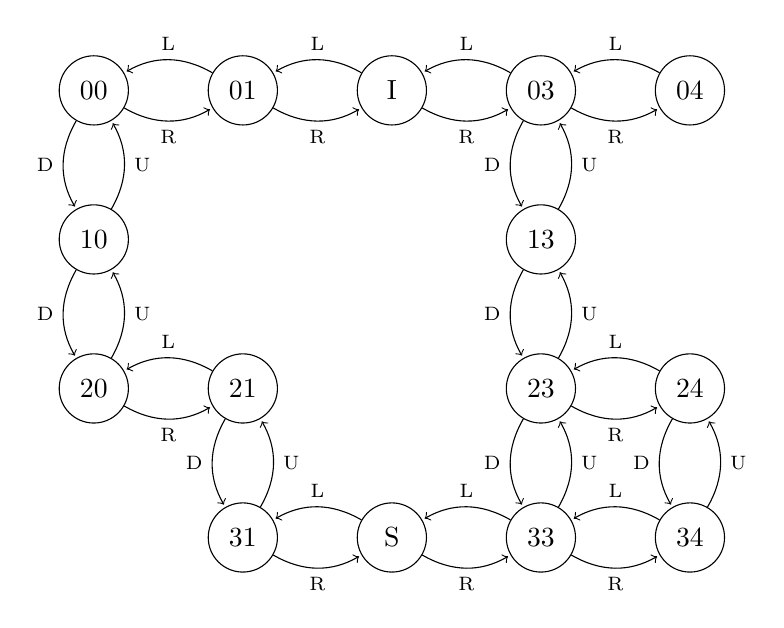
\begin{tikzpicture}
        % Draw the states
        \node[state]                (00) {00};
        \node[state, right=of 00]   (01) {01};
        \node[state, right=of 01]   (i)  {I};
        \node[state, right=of i]    (03) {03};
        \node[state, right=of 03]   (04) {04};
    
        \node[state, below=of 00]  (10) {10};
        \node[state, below=of 03]  (13) {13};
    
        \node[state, below=of 10]  (20) {20};
        \node[state, right=of 20]  (21) {21};
        \node[state, below=of 13]  (23) {23};
        \node[state, right=of 23]  (24) {24};
    
        \node[state, below=of 21]  (31) {31};
        \node[state, right=of 31]  (s) {S};
        \node[state, right=of s]   (33) {33};
        \node[state, right=of 33]  (34) {34};
    
        % Connect the states with arrows
        \draw[every loop]
            (00) edge[bend right, auto=right] node {\scriptsize R} (01)
            (01) edge[bend right, auto=right] node {\scriptsize L} (00)
            (01) edge[bend right, auto=right] node {\scriptsize R} (i)
            (i) edge[bend right, auto=right] node {\scriptsize L} (01)
            (i) edge[bend right, auto=right] node {\scriptsize R} (03)
            (03) edge[bend right, auto=right] node {\scriptsize L} (i)
            (03) edge[bend right, auto=right] node {\scriptsize R} (04)
            (04) edge[bend right, auto=right] node {\scriptsize L} (03)

            (00) edge[bend right, auto=right] node {\scriptsize D} (10)
            (10) edge[bend right, auto=right] node {\scriptsize U} (00)
            (03) edge[bend right, auto=right] node {\scriptsize D} (13)
            (13) edge[bend right, auto=right] node {\scriptsize U} (03)

            (10) edge[bend right, auto=right] node {\scriptsize D} (20)
            (20) edge[bend right, auto=right] node {\scriptsize U} (10)
            (13) edge[bend right, auto=right] node {\scriptsize D} (23)
            (23) edge[bend right, auto=right] node {\scriptsize U} (13)

            (20) edge[bend right, auto=right] node {\scriptsize R} (21)
            (21) edge[bend right, auto=right] node {\scriptsize L} (20)
            (23) edge[bend right, auto=right] node {\scriptsize R} (24)
            (24) edge[bend right, auto=right] node {\scriptsize L} (23)

            (21) edge[bend right, auto=right] node {\scriptsize D} (31)
            (31) edge[bend right, auto=right] node {\scriptsize U} (21)
            (23) edge[bend right, auto=right] node {\scriptsize D} (33)
            (33) edge[bend right, auto=right] node {\scriptsize U} (23)
            (24) edge[bend right, auto=right] node {\scriptsize D} (34)
            (34) edge[bend right, auto=right] node {\scriptsize U} (24)

            (31) edge[bend right, auto=right] node {\scriptsize R} (s)
            (s) edge[bend right, auto=right] node {\scriptsize L} (31)
            (s) edge[bend right, auto=right] node {\scriptsize R} (33)
            (33) edge[bend right, auto=right] node {\scriptsize L} (s)
            (33) edge[bend right, auto=right] node {\scriptsize R} (34)
            (34) edge[bend right, auto=right] node {\scriptsize L} (33);
    \end{tikzpicture}
\end{adjustbox}
\caption{MDP determinista}
\end{figure}

\p{Así pues, el MDP queda como se muestra en la figura superior. Las acciones posibles son Izquierda (L), Derecha (R), Arriba (U) y Abajo (D).}

\subsection{10. ¿Cuántos ciclos crees que serán necesarios para aprender la política optima?¿Por qué?}
\p{Se necesitarán al menos 5 ciclos, ya que es la distancia mínima (5 acciones o transiciones) desde el origen a la meta, todas las acciones son deterministas, no hay acciones con refuerzo negativo, y las únicas acciones con refuerzo positivo son las que transitan al estado meta desde algún estado vecino.}
\p{Por ello, para que el refuerzo de la acción ``L'' del nodo 33 al nodo ``S'' (la más cercana de las dos únicas acciones con refuerzo positivo) se propague hasta las acciones posibles en el nodo ``I'' serán necesarios cinco ciclos.}

\subsection{11. Generar la tabla Q ejecutando el código anterior y responder a las siguientes preguntas:}
\p{Se ha generado la siguiente tabla. En verde se muestran el estado inicial y estado meta. En rojo se muestran las acciones elegidas por la política generada.}
\begin{table}[h!]
    \label{tablaqdet}
    \centering
    \begin{tabular}{c|c|c|c|c|}
    \cline{2-5}
    S/A                                             & L                            & R                            & U    & D                            \\ \hline
    \multicolumn{1}{|c|}{00}                        & 0.0                          & 0.0                          & 0.0  & 0.41                         \\ \hline
    \multicolumn{1}{|c|}{01}                        & 0.0                          & 0.0                          & 0.0  & 0.0                          \\ \hline
    \rowcolor[HTML]{9AFF99} 
    \multicolumn{1}{|c|}{\cellcolor[HTML]{9AFF99}I} & 0.0                          & \cellcolor[HTML]{FD6864}0.67 & 0.0  & 0.0                          \\ \hline
    \multicolumn{1}{|c|}{03}                        & 0.54                         & 0.0                          & 0.0  & \cellcolor[HTML]{FD6864}1.05 \\ \hline
    \multicolumn{1}{|c|}{04}                        & 0.67                         & 0.0                          & 0.0  & 0.0                          \\ \hline
    \multicolumn{1}{|c|}{10}                        & 0.0                          & 0.0                          & 0.33 & 0.84                         \\ \hline
    \multicolumn{1}{|c|}{13}                        & 0.0                          & 0.0                          & 0.84 & \cellcolor[HTML]{FD6864}1.48 \\ \hline
    \multicolumn{1}{|c|}{20}                        & 0.0                          & 1.31                         & 0.67 & 0.0                          \\ \hline
    \multicolumn{1}{|c|}{21}                        & 1.05                         & 0.0                          & 0.0  & 1.85                         \\ \hline
    \multicolumn{1}{|c|}{23}                        & 0.0                          & 1.18                         & 1.18 & \cellcolor[HTML]{FD6864}1.95 \\ \hline
    \multicolumn{1}{|c|}{24}                        & 1.48                         & 0.0                          & 0.0  & 1.59                         \\ \hline
    \multicolumn{1}{|c|}{31}                        & 0.0                          & 2.48                         & 1.48 & 0.0                          \\ \hline
    \rowcolor[HTML]{9AFF99} 
    \multicolumn{1}{|c|}{\cellcolor[HTML]{9AFF99}S} & 1.98                         & 1.98                         & 0.0  & 0.0                          \\ \hline
    \multicolumn{1}{|c|}{33}                        & \cellcolor[HTML]{FD6864}2.59 & 1.59                         & 1.59 & 0.0                          \\ \hline
    \multicolumn{1}{|c|}{34}                        & 2.07                         & 0.0                          & 1.27 & 0.0                          \\ \hline
    \end{tabular}
    \caption{Tabla Q MDP determinista para 5 ciclos, $\alpha$ = 1.0, $\gamma$ = 0.8}
\end{table}
\subsubsection{a) ¿Qué alfa y gamma has utilizado? ¿Por qué?}
\p{Hemos utilizado un valor de alfa de 1,0 y un valor de gamma de 0,8.}
\p{Hemos situado alfa a su máximo valor dado que todas las acciones posibles son deterministas, por lo que el ratio de aprendizaje del agente será constante. Por este motivo y en este caso, un valor máximo de alfa ayuda a ajustar antes los valores de refuerzo de la política con mayor precisión.}
\p{Hemos elegido un valor elevado para gamma buscando favorecer y potenciar el refuerzo futuro, acelerando la propagación de este. En realidad y para este caso, cualquier valor elevado funcionaría bastante bien (mejor que un valor gamma reducido), ya que todas las acciones son deterministas, no hay acciones con refuerzo negativo, y las únicas acciones con refuerzo positivo son las que transitan al estado meta desde algún estado vecino.}

\subsubsection{b) ¿Se genera la política óptima?}
\p{Sí, el agente realiza el camino más corto que consiste en el siguiente:}
\newpage
\begin{figure}[h!]\label{politica}
% Grid
\begin{adjustbox}{valign=m,minipage={0.4\linewidth}}
    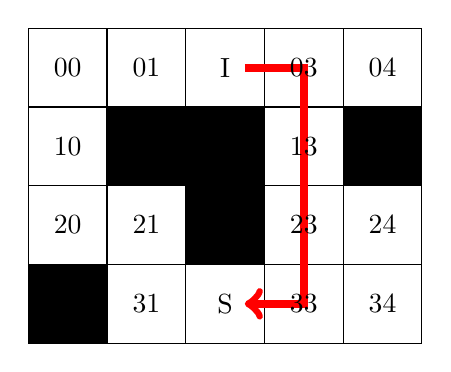
\begin{tikzpicture}
        % Pintar grid
        \draw[step=1cm,black] (0,0) grid (5,4);
        % Poner los muros de negro (casillas negras)
        \fill[black] (0,0) rectangle (1,1);
        \fill[black] (1,2) rectangle (2,3);
        \fill[black] (2,2) rectangle (3,3);
        \fill[black] (2,1) rectangle (3,2);
        \fill[black] (4,2) rectangle (5,3);
        % Camino en rojo
        \draw[red,line width=1mm, ->] (2.75,3.5) -- (3.5,3.5) -- (3.5,2.5) -- (3.5,1.5) -- (3.5,0.5) -- (2.75,0.5);
        % Texto de las casillas
        \node at (0.5,3.5) {00};
        \node at (1.5,3.5) {01};
        \node at (2.5,3.5) {I};
        \node at (3.5,3.5) {03};
        \node at (4.5,3.5) {04};

        \node at (0.5,2.5) {10};
        \node at (3.5,2.5) {13};

        \node at (0.5,1.5) {20};
        \node at (1.5,1.5) {21};
        \node at (3.5,1.5) {23};
        \node at (4.5,1.5) {24};

        \node at (1.5,0.5) {31};
        \node at (2.5,0.5) {S};
        \node at (3.5,0.5) {33};
        \node at (4.5,0.5) {34};
    \end{tikzpicture}
    % \hspace{1cm}
\end{adjustbox}
% MDP
\begin{adjustbox}{valign=m,minipage={0.4\linewidth}}
    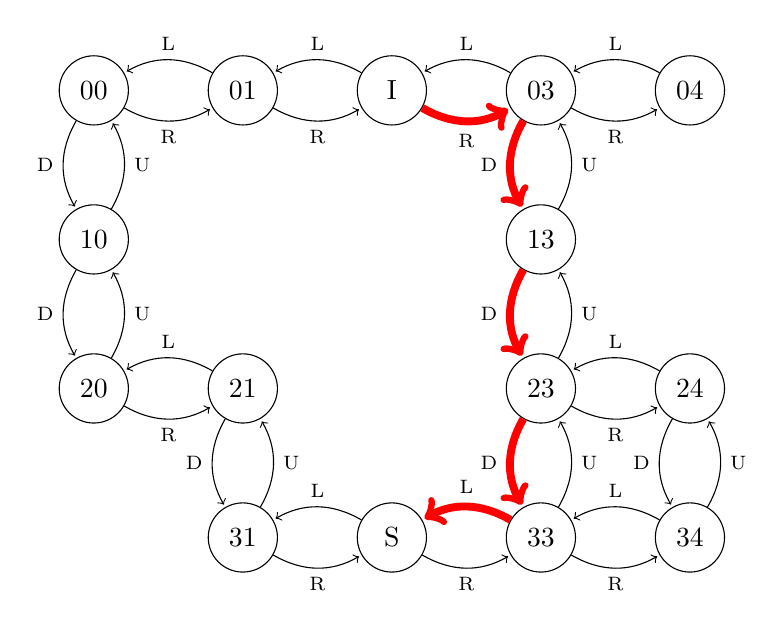
\begin{tikzpicture}
        % Draw the states
        \node[state]                (00) {00};
        \node[state, right=of 00]   (01) {01};
        \node[state, right=of 01]   (i)  {I};
        \node[state, right=of i]    (03) {03};
        \node[state, right=of 03]   (04) {04};
    
        \node[state, below=of 00]  (10) {10};
        \node[state, below=of 03]  (13) {13};
    
        \node[state, below=of 10]  (20) {20};
        \node[state, right=of 20]  (21) {21};
        \node[state, below=of 13]  (23) {23};
        \node[state, right=of 23]  (24) {24};
    
        \node[state, below=of 21]  (31) {31};
        \node[state, right=of 31]  (s) {S};
        \node[state, right=of s]   (33) {33};
        \node[state, right=of 33]  (34) {34};
    
        % Connect the states with arrows
        \draw[every loop]
            (00) edge[bend right, auto=right] node {\scriptsize R} (01)
            (01) edge[bend right, auto=right] node {\scriptsize L} (00)
            (01) edge[bend right, auto=right] node {\scriptsize R} (i)
            (i) edge[bend right, auto=right] node {\scriptsize L} (01)
            (03) edge[bend right, auto=right] node {\scriptsize L} (i)
            (03) edge[bend right, auto=right] node {\scriptsize R} (04)
            (04) edge[bend right, auto=right] node {\scriptsize L} (03)

            (00) edge[bend right, auto=right] node {\scriptsize D} (10)
            (10) edge[bend right, auto=right] node {\scriptsize U} (00)
            (13) edge[bend right, auto=right] node {\scriptsize U} (03)

            (10) edge[bend right, auto=right] node {\scriptsize D} (20)
            (20) edge[bend right, auto=right] node {\scriptsize U} (10)
            (23) edge[bend right, auto=right] node {\scriptsize U} (13)

            (20) edge[bend right, auto=right] node {\scriptsize R} (21)
            (21) edge[bend right, auto=right] node {\scriptsize L} (20)
            (23) edge[bend right, auto=right] node {\scriptsize R} (24)
            (24) edge[bend right, auto=right] node {\scriptsize L} (23)

            (21) edge[bend right, auto=right] node {\scriptsize D} (31)
            (31) edge[bend right, auto=right] node {\scriptsize U} (21)
            (33) edge[bend right, auto=right] node {\scriptsize U} (23)
            (24) edge[bend right, auto=right] node {\scriptsize D} (34)
            (34) edge[bend right, auto=right] node {\scriptsize U} (24)

            (31) edge[bend right, auto=right] node {\scriptsize R} (s)
            (s) edge[bend right, auto=right] node {\scriptsize L} (31)
            (s) edge[bend right, auto=right] node {\scriptsize R} (33)
            (33) edge[bend right, auto=right] node {\scriptsize R} (34)
            (34) edge[bend right, auto=right] node {\scriptsize L} (33);

            \draw[every loop,line width=1mm,draw=red]
            (i) edge[bend right, auto=right] node {\scriptsize R} (03)
            (03) edge[bend right, auto=right] node {\scriptsize D} (13)
            (13) edge[bend right, auto=right] node {\scriptsize D} (23)
            (23) edge[bend right, auto=right] node {\scriptsize D} (33)
            (33) edge[bend right, auto=right] node {\scriptsize L} (s);
    \end{tikzpicture}
\end{adjustbox}
\caption{Política MDP determinista}
\end{figure}
\vspace{-2em}
\subsubsection{c) ¿Cuántos ciclos se necesitan para obtener la política óptima y cuál es esta política?}
\p{Como se ha explicado en diversos apartados anteriores. El agente es capaz de calcular la política óptima en 5 ciclos como mínimo, y dicha política es la representada en la imagen superior, así como en la \customref{tablaqdet}{tabla Q anterior}.}

\section{MDP estocástico}
\vspace{-1em}
\subsection{12. Ilustración del modelo}
\p{El MDP sigue siendo prácticamente el mismo, pues la mayoría de acciones transitan al estado correspondiente con probabilidad 1. Solo la acción Izquierda (L) del estado 33 es no determinista. Se refleja este cambio en rojo en la siguiente imagen.}

\begin{figure}[h!]
% Grid
\vspace{-2em}
\begin{adjustbox}{valign=m,minipage={0.4\linewidth}}
    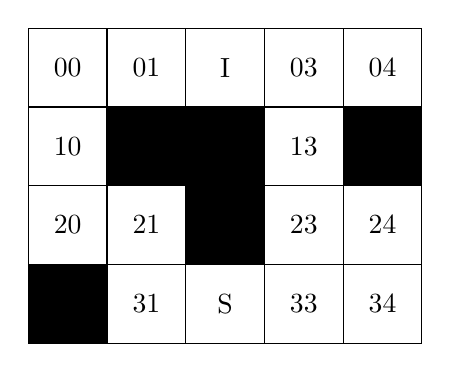
\begin{tikzpicture}
        % Pintar grid
        \draw[step=1cm,black] (0,0) grid (5,4);
        % Poner los muros de negro (casillas negras)
        \fill[black] (0,0) rectangle (1,1);
        \fill[black] (1,2) rectangle (2,3);
        \fill[black] (2,2) rectangle (3,3);
        \fill[black] (2,1) rectangle (3,2);
        \fill[black] (4,2) rectangle (5,3);
        % Texto de las casillas
        \node at (0.5,3.5) {00};
        \node at (1.5,3.5) {01};
        \node at (2.5,3.5) {I};
        \node at (3.5,3.5) {03};
        \node at (4.5,3.5) {04};

        \node at (0.5,2.5) {10};
        \node at (3.5,2.5) {13};

        \node at (0.5,1.5) {20};
        \node at (1.5,1.5) {21};
        \node at (3.5,1.5) {23};
        \node at (4.5,1.5) {24};

        \node at (1.5,0.5) {31};
        \node at (2.5,0.5) {S};
        \node at (3.5,0.5) {33};
        \node at (4.5,0.5) {34};
    \end{tikzpicture}
    % \hspace{1cm}
\end{adjustbox}
% MDP
\begin{adjustbox}{valign=m,minipage={0.4\linewidth}}
    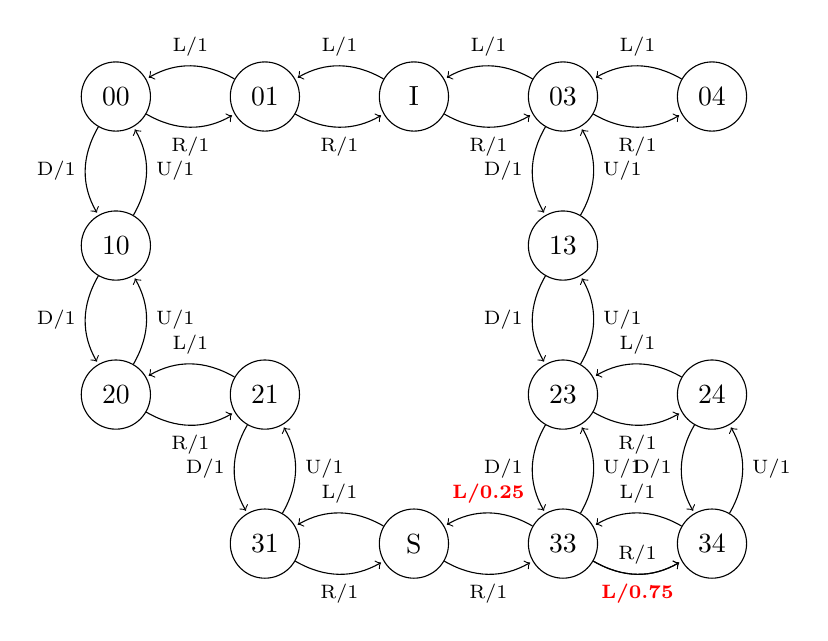
\begin{tikzpicture}
        % Draw the states
        \node[state]                (00) {00};
        \node[state, right=of 00]   (01) {01};
        \node[state, right=of 01]   (i)  {I};
        \node[state, right=of i]    (03) {03};
        \node[state, right=of 03]   (04) {04};
    
        \node[state, below=of 00]  (10) {10};
        \node[state, below=of 03]  (13) {13};
    
        \node[state, below=of 10]  (20) {20};
        \node[state, right=of 20]  (21) {21};
        \node[state, below=of 13]  (23) {23};
        \node[state, right=of 23]  (24) {24};
    
        \node[state, below=of 21]  (31) {31};
        \node[state, right=of 31]  (s) {S};
        \node[state, right=of s]   (33) {33};
        \node[state, right=of 33]  (34) {34};
    
        % Connect the states with arrows
        \draw[every loop]
            (00) edge[bend right, auto=right] node {\scriptsize R/1} (01)
            (01) edge[bend right, auto=right] node {\scriptsize L/1} (00)
            (01) edge[bend right, auto=right] node {\scriptsize R/1} (i)
            (i) edge[bend right, auto=right] node {\scriptsize L/1} (01)
            (i) edge[bend right, auto=right] node {\scriptsize R/1} (03)
            (03) edge[bend right, auto=right] node {\scriptsize L/1} (i)
            (03) edge[bend right, auto=right] node {\scriptsize R/1} (04)
            (04) edge[bend right, auto=right] node {\scriptsize L/1} (03)

            (00) edge[bend right, auto=right] node {\scriptsize D/1} (10)
            (10) edge[bend right, auto=right] node {\scriptsize U/1} (00)
            (03) edge[bend right, auto=right] node {\scriptsize D/1} (13)
            (13) edge[bend right, auto=right] node {\scriptsize U/1} (03)

            (10) edge[bend right, auto=right] node {\scriptsize D/1} (20)
            (20) edge[bend right, auto=right] node {\scriptsize U/1} (10)
            (13) edge[bend right, auto=right] node {\scriptsize D/1} (23)
            (23) edge[bend right, auto=right] node {\scriptsize U/1} (13)

            (20) edge[bend right, auto=right] node {\scriptsize R/1} (21)
            (21) edge[bend right, auto=right] node {\scriptsize L/1} (20)
            (23) edge[bend right, auto=right] node {\scriptsize R/1} (24)
            (24) edge[bend right, auto=right] node {\scriptsize L/1} (23)

            (21) edge[bend right, auto=right] node {\scriptsize D/1} (31)
            (31) edge[bend right, auto=right] node {\scriptsize U/1} (21)
            (23) edge[bend right, auto=right] node {\scriptsize D/1} (33)
            (33) edge[bend right, auto=right] node {\scriptsize  U/1} (23)
            (24) edge[bend right, auto=right] node {\scriptsize  D/1} (34)
            (34) edge[bend right, auto=right] node {\scriptsize U/1} (24)

            (31) edge[bend right, auto=right] node {\scriptsize R/1} (s)
            (s) edge[bend right, auto=right] node {\scriptsize L/1} (31)
            (s) edge[bend right, auto=right] node {\scriptsize R/1} (33)
            (33) edge[bend right, auto=right] node {\scriptsize \color{red}\textbf{L/0.25}} (s)
            (33) edge[bend right, auto=right] node {\scriptsize \color{red}\textbf{L/0.75}} (34)
            (33) edge[bend right, auto=left] node {\scriptsize R/1} (34)
            (34) edge[bend right, auto=right] node {\scriptsize L/1} (33);
    \end{tikzpicture}
\end{adjustbox}
\caption{MDP \textbf{NO} determinista}
\end{figure}

\subsection{13. Generar las tuplas de todos los episodios para el problema del apartado anterior y generar la tabla Q utilizando distintos valores para alfa y gamma. Responder a las siguientes preguntas:}
\p{Respecto al MDP anterior, se ha modificado el código de \texttt{main.java} para incluir 4 tuplas para el estado 33 y la acción ``L''. Tres de estas tuplas transitan al estado ``34'' (probabilidad 0.75) y solo la tupla restante transita al estado ``S'' (probabilidad 0.25). }
\p{Al igual que en la tabla anterior, se muestran en verde el estado inicial y estado meta y en rojo las acciones elegidas por la política generada.}
\begin{table}[h!]
    \label{tablaqestoc}
    \centering
    \begin{tabular}{c|c|c|c|c|}
    \cline{2-5}
    S/A                                             & L                            & R                            & U    & D                            \\ \hline
    \multicolumn{1}{|c|}{00}                        & 0.0                          & 0.0                          & 0.0  & 0.01                         \\ \hline
    \multicolumn{1}{|c|}{01}                        & 0.0                          & 0.0                          & 0.0  & 0.0                          \\ \hline
    \rowcolor[HTML]{9AFF99} 
    \multicolumn{1}{|c|}{\cellcolor[HTML]{9AFF99}I} & 0.0                          & \cellcolor[HTML]{FD6864}0.02 & 0.0  & 0.0                          \\ \hline
    \multicolumn{1}{|c|}{03}                        & 0.01                         & 0.0                          & 0.0  & \cellcolor[HTML]{FD6864}0.17 \\ \hline
    \multicolumn{1}{|c|}{04}                        & 0.02                         & 0.0                          & 0.0  & 0.0                          \\ \hline
    \multicolumn{1}{|c|}{10}                        & 0.0                          & 0.0                          & 0.01 & 0.1                         \\ \hline
    \multicolumn{1}{|c|}{13}                        & 0.0                          & 0.0                          & 0.08 & \cellcolor[HTML]{FD6864}0.57 \\ \hline
    \multicolumn{1}{|c|}{20}                        & 0.0                          & 0.37                         & 0.05 & 0.0                          \\ \hline
    \multicolumn{1}{|c|}{21}                        & 0.2                         & 0.0                          & 0.0  & 0.86                         \\ \hline
    \multicolumn{1}{|c|}{23}                        & 0.0                          & 0.31                         & 0.31 & \cellcolor[HTML]{FD6864}1.19 \\ \hline
    \multicolumn{1}{|c|}{24}                        & 0.57                         & 0.0                          & 0.0  & 0.76                         \\ \hline
    \multicolumn{1}{|c|}{31}                        & 0.0                          & 1.55                         & 0.53 & 0.0                          \\ \hline
    \rowcolor[HTML]{9AFF99} 
    \multicolumn{1}{|c|}{\cellcolor[HTML]{9AFF99}S} & 1.05                         & 1.19                         & 0.0  & 0.0                          \\ \hline
    \multicolumn{1}{|c|}{33}                        & \cellcolor[HTML]{FD6864}1.94 & 0.76                         & 0.76 & 0.0                          \\ \hline
    \multicolumn{1}{|c|}{34}                        & 1.37                         & 0.0                          & 0.46 & 0.0                          \\ \hline
    \end{tabular}
    \caption{Tabla Q MDP \textbf{NO} determinista para 5 ciclos, $\alpha$ = 0.5, $\gamma$ = 0.8}
\end{table}

\subsubsection{a) ¿Qué valores has utilizado para alfa y gamma y por qué esos valores?. Intenta explicar para qué sirven alfa y gamma.}
\p{Hemos utilizado un valor de alfa de 0,5 y un valor de gamma de 0,8.}
\p{Hemos situado alfa a un valor medio dado que \textbf{no} todas las acciones posibles son deterministas, por lo que queremos ``filtrar'' el ratio de aprendizaje del agente. Con este valor, que es distinto de 1, conseguimos que el agente tenga en cuenta no solo el refuerzo conseguido en cada ciclo, sino también el refuerzo conseguido en ciclos anteriores.}
\p{Hemos elegido un valor elevado para gamma buscando favorecer y potenciar el refuerzo futuro, acelerando la propagación de este. En realidad y para este caso, cualquier valor elevado funcionaría bastante bien (mejor que un valor gamma reducido), ya que \textbf{casi} todas las acciones son deterministas, no hay acciones con refuerzo negativo, y las únicas acciones con refuerzo positivo son las que transitan al estado meta desde algún estado vecino.}
\p{Así pues, podemos concluir que \textbf{alfa es el ratio de aprendizaje del agente}, determina hasta que punto la nueva información sustituye a la anterior, siendo este ritmo de sustitución mayor cuanto más elevado es el valor de alfa. Por otra parte, \textbf{gamma es el factor de descuento del refuerzo} o recompensa, y determina la importancia de recompensas futuras.}
\p{Los valores límite de estos parámetros afectan al aprendizaje de la siguiente forma:}
\begin{itemize}
    \item \textbf{$\bm{\alpha}$ = 1:} la información nueva sustituye por completo a la información conocida, común en los MDP deterministas.
    \item \textbf{$\bm{\alpha}$ = 0:} no se sustituye nunca la información conocida inicialmente por el agente, por lo que este no aprende nada.
    \item \textbf{$\bm{\gamma}$ = 1:} fomenta el aprendizaje de comportamientos que reportan recompensa a largo plazo.
    \item \textbf{$\bm{\gamma}$ = 0:} fomenta el aprendizaje de comportamientos que reportan recompensa inmediata.
\end{itemize}

\subsubsection{b) ¿Qué diferencias hay entre las distintas tablas Q y las políticas obtenidas?}
\p{La política obtenida es exactamente la misma que para el MDP determinista, al menos con los valores de $\alpha$ = 0.5 y $\gamma$ = 0.8 utilizados para la generación de la \customref{tablaqestoc}{tabla anterior}, independientemente del número de ciclos (con ciclos $\geq$ 5). Esta política se puede visualizar sobre el tablero y el grafo del MDP determinista en la \customref{politica}{imagen de política} de dicho MDP, pues reincidimos en que esta política es la misma.}
\p{Sin embargo, si comprobamos ambas tablas, vemos que en general el valor-acción es menor en todos los casos en la \customref{tablaqestoc}{tabla del MDP \textbf{no} determinista} frente a la \customref{tablaqdet}{tabla del MDP determinista}. Esto se debe principalmente a que estamos filtrando el aprendizaje mediante un valor de alfa menor que 1, y a que la baja probabilidad con la que se transita del estado ``33'' al estado ``S'' con la acción ``L'' (que forma parte de la política) provoca una notoria reducción del refuerzo conseguido en dicha situación, lo que afecta a su propagación hacia el estado ``I''.}

\section{Material entregado}
\p{Junto a esta memoria se entrega el código utilizado para la realización del tutorial 4. Este código es el mismo que ha sido descargado de Aula Global, y solo se ha modificado el fichero \texttt{main.java}.}
\p{Concretamente, el contenido de los arrays \texttt{acciones} (línea 21), \texttt{estados} (22), \texttt{estado} (24), \texttt{estadoFinal} (25), los parámetros pasados al constructor de \texttt{QLearning} en la instanciación de \texttt{ql} (31) y las tuplas de la línea 36 a la 70.}
\p{Se entrega el código en el mismo estado en el que se encontraba tras terminar este tutorial. Esto es, tras realizar el algoritmo de Q-learning sobre el MDP no de terminista o estocástico.}

\section{Problemas encontrados a la hora de realizar este tutorial}
\p{El único problema encontrado durante la realización de este tutorial ha sido a la hora de generar las transiciones del MDP estocástico en el código java proporcionado. No hemos encontrado en el código ni los comentarios del fichero \texttt{main.java} ni del resto de ficheros una opción para indicar la probabilidad de las transiciones, que nos ha sido necesario para la acción ``L'' en el estado ``33''. Tampoco hemos encontrado documentación o información acerca de este paso en el enunciado, o si estaba, esta no era clara.}
\p{Finalmente se ha optado por incluir 4 tuplas para la acción ``L'' en el estado ``33''. Tres tuplas que transitan hacia el estado ``34'' (probabilidad de 0.75) y una sola que transita al estado ``S'' (probabilidad de 0.25). De esta forma se ha intentado emular el no determinismo de la acción.}

\section{Conclusiones}
\p{En general, este ha sido un tutorial fácil y que nos va a ayudar de cara a la realización de la próxima práctica, en la que tendremos que programar un agente inteligente de Mario que aprenda por refuerzo. El completar este tutorial nos ha permitido comprender mejor el funcionamiento del algoritmo de aprendizaje por refuerzo \textit{Q-Learning}, así como la importancia y el papel que juegan en el mismo los parámetros alfa y gama.}

\section{Comentarios personales}
\p{Hemos tardado entre 3 y 4 horas en la realización de este tutorial, mucho más allá de la duración de una hora que se indicaba en la cabecera del enunciado. Asimismo, hemos preguntado a algunos de nuestros compañeros y coincidían con nosotros en que el tiempo empelado en la realización del tutorial ha sido mayor que el indicado.}
\p{Creemos que esto se debe a varios factores, como son:}
\begin{itemize}
    \item Tiempo empleado en el siempre necesario repaso de la teoría de la asignatura.
    \item Tiempo empleado en entender el código proporcionado que ha sido programado por un tercero.
    \item Tiempo empleado en la experimentación (que a veces va acompañado de una investigación, ya sea un repaso de la teoría más lento y detallado o búsquedas en Internet).
    \item Tiempo empleado en la documentación de la práctica, teniendo en cuenta revisiones ortográficas y de formato, y atendiendo a la corrección de las respuestas.
    \item Asimismo, el tiempo empleado en entender algunos comentarios del enunciado, cuyas explicaciones en ocasiones resultan ambiguas o poco clara, lo cual entendemos que es difícil de detectar para la persona que lo escribe y dada en ocasiones la diferencia de entrenamiento o conocimiento en el tipo de trabajo a realizar.
\end{itemize}
\p{Tenemos la sensación de que no se se tiene en cuenta, probablemente por desconocimiento, el verdadero trabajo que hay detrás de una tarea aparentemente (y que de hecho es) fácil, como es este tutorial. Esto induce a un mal cálculo o aproximación, que sumado a la carga de trabajo del resto de asignaturas, en ocasiones nos impide dedicarle el tiempo y esfuerzo que nos gustaría a estas prácticas.}

\end{document}